%\documentclass{article}
%\usepackage{graphicx,subfigure}
%\begin{document}

\begin{figure}[!h]
  \centering
   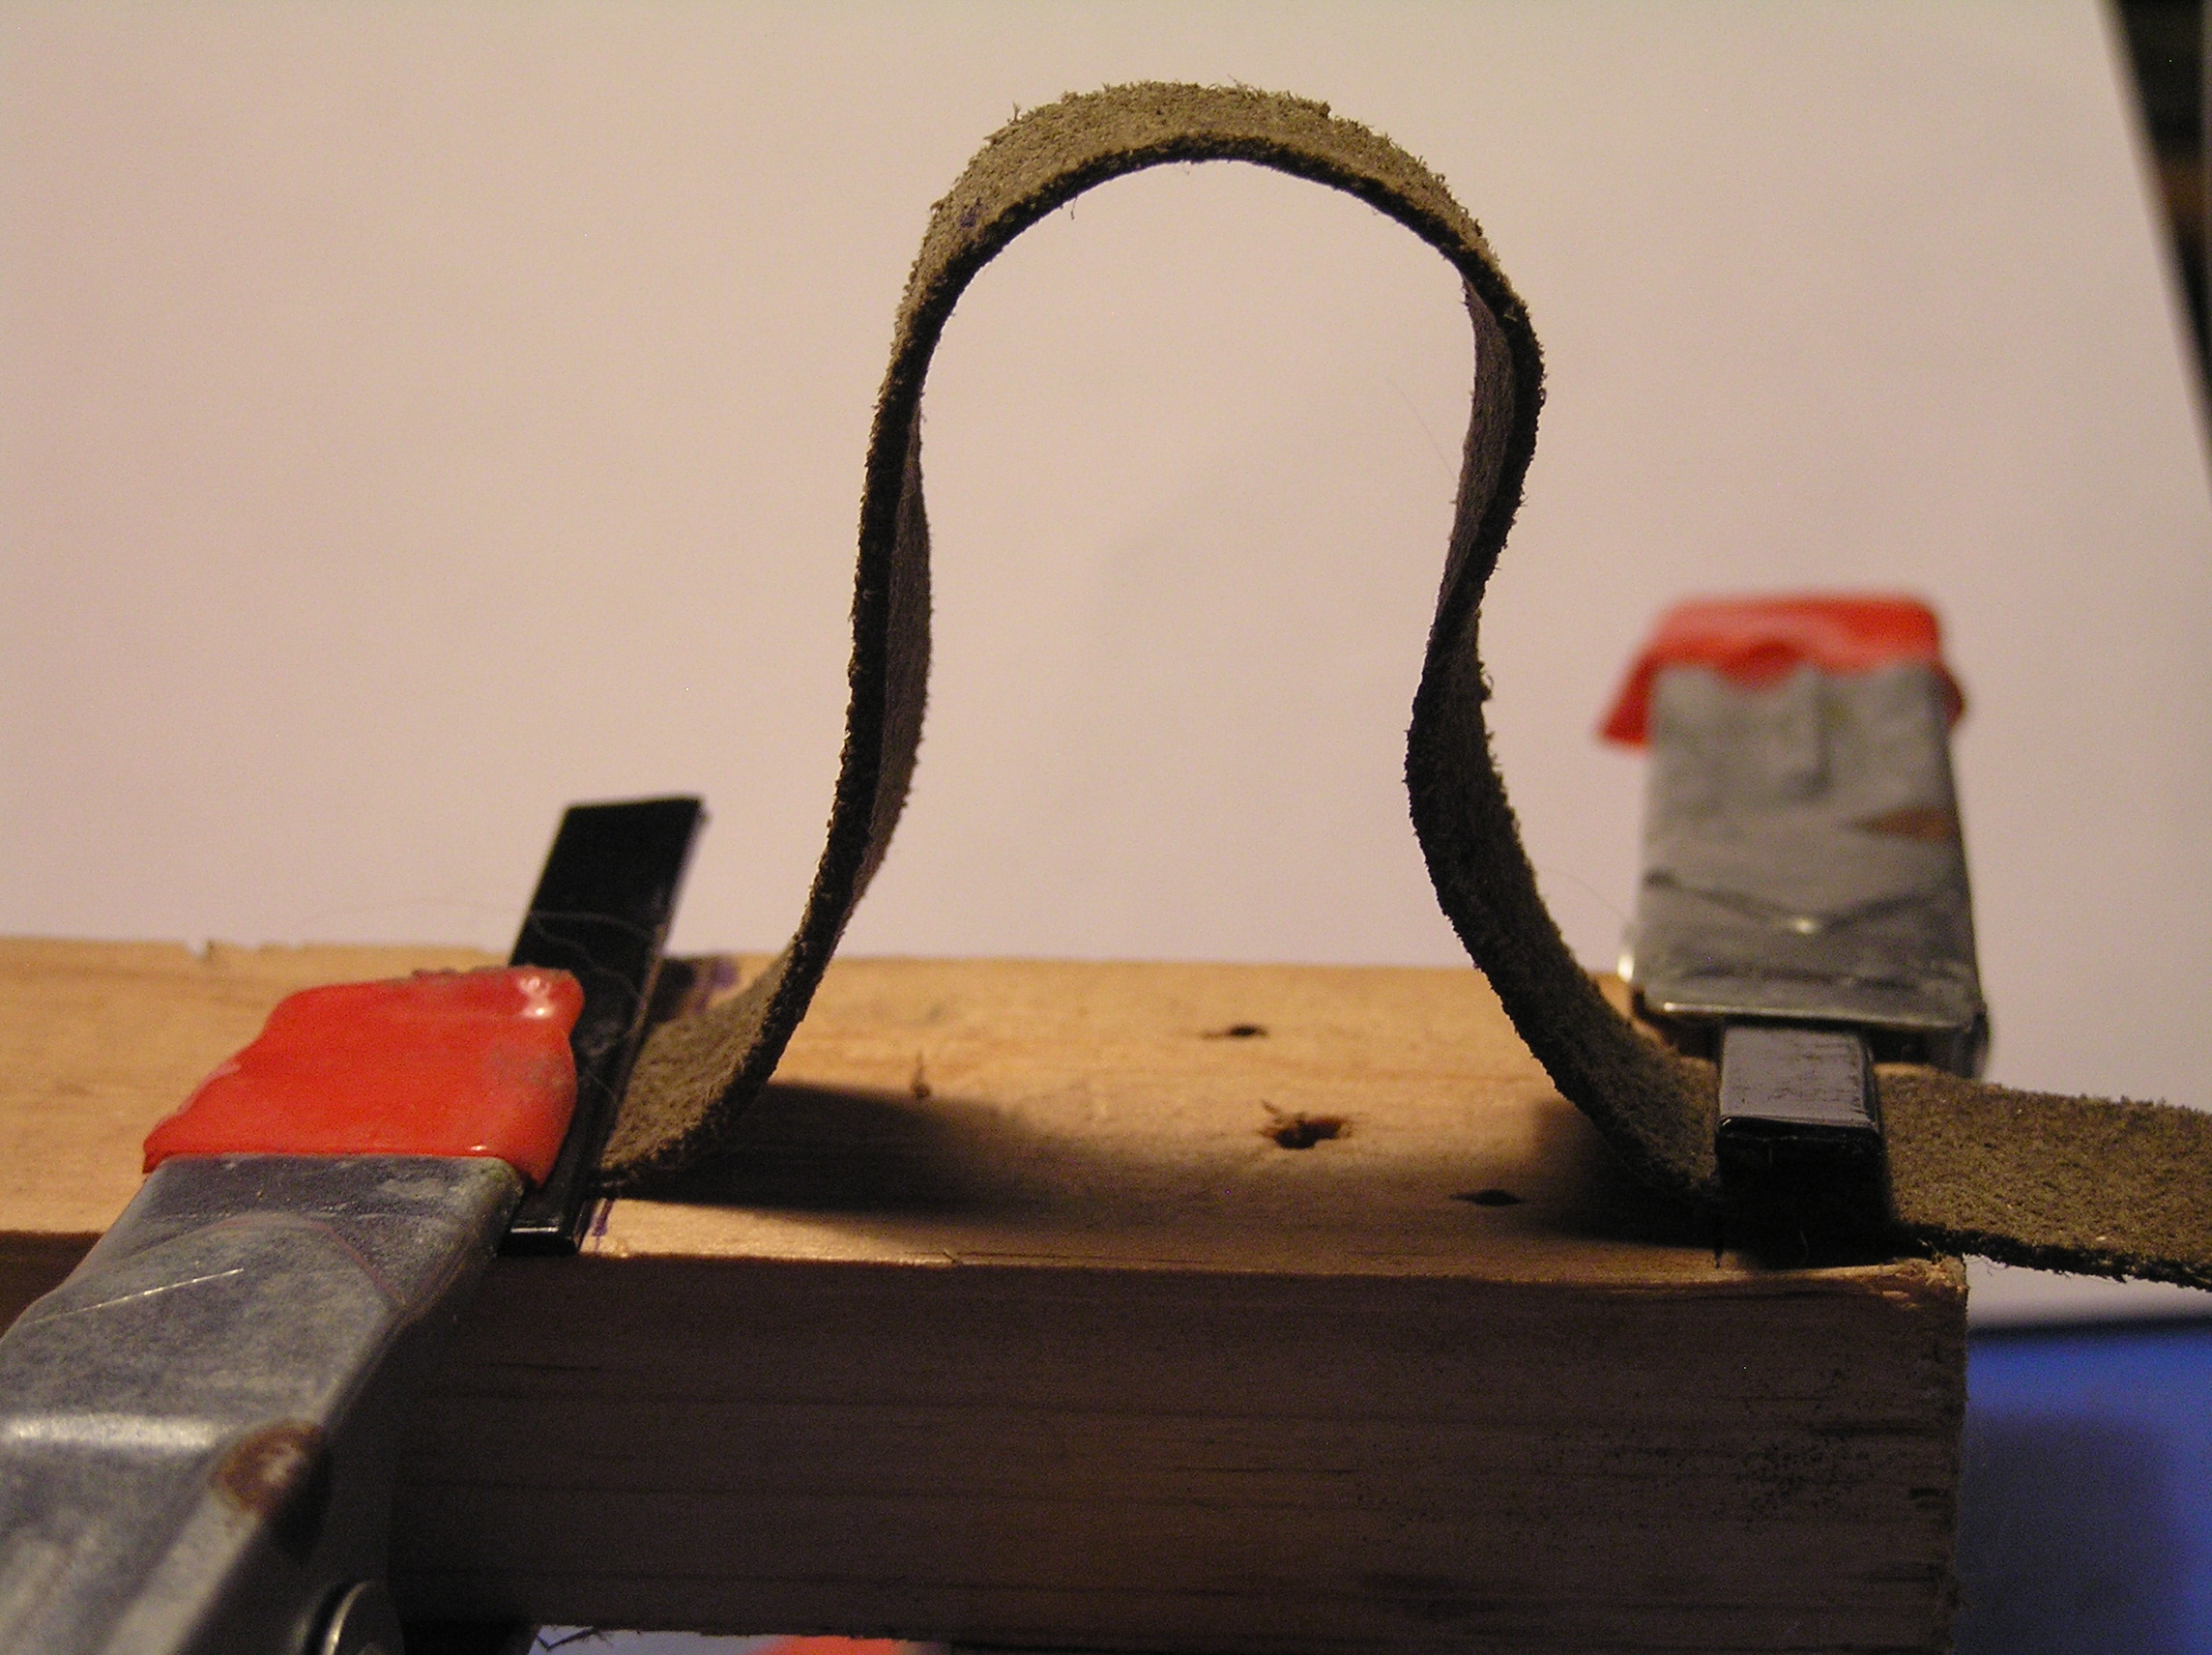
\includegraphics[width=0.9\textwidth]{images/P1010019.JPG}
  \caption{Physical model with a 50mm strip of leather clamped at 0mm and 120 to a board at positions 0 and 50mm. The leather represents dermis. The board represents subdermal tissue. This demonstrates fold formation when the leather strip has 70mm of expansion (over the original 50mm), a 140 percent expansion.}
  \label{fig:model4}
\end{figure}

%\end{document}

